\section{Suggestions to Improve the Existing System}

\subsection{System Perspective}

% Checked in grammarly
\afetbilgi is not part of a more extensive system. It is a standalone and open-source efforted website to verify critical information in the fight against the 6 February 2023 Pazarcik Earthquake and deliver it to disaster victims and those who want to help in an understandable, concise manner in multiple languages.

This information is presented in either the form of legible tables with third-party governmental and private links or an interactable method via a map view interface. If deemed necessary, admin and maintainers can make changes to display newly created or edited data and upload it to the system upon any complaints or suggestions they may get on their contact details.

\begin{figure}[H]
  \centering
  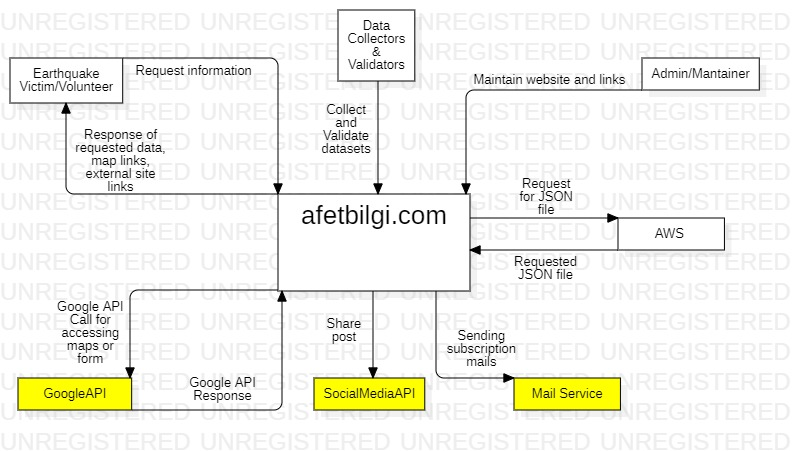
\includegraphics[width=\linewidth]{img/context-diagram-s4.jpg}
  \caption{Context Diagram for \afetbilgi}
\end{figure}

\vfill
\newpage

The \afetbilgi\ consists of a combination of small physical and software parts. With the help of interfaces, these parts communicate among themselves and with the user. The following are the interfaces through which interaction occurs:
\begin{itemize}
  \setlength{\itemsep}{1pt}
  \item User interfaces
  \item Software interfaces
  \item Communication interfaces
\end{itemize}
Users interact with the website through their devices connected to the internet, such as cell phones or computers, as the user interface. The software interface enables the website to serve additional features to the user.

\subsubsection{User Interfaces}

In order to start using the website, a user should go into the website via a device connected to the internet. The website may have some loading time. After loading, the website is ready for user interactions. Users can interact with \afetbilgi\ directly to access required information.

The user interface contains \href{https://mui.com/}{MUI} components which are clear buttons and lists. Users can interact with the buttons to access the list of information or access more options related to the chosen information type.

\subsubsection{Software Interfaces}

\afetbilgi\ runs mainly JavaScript code with React library. It also uses additional react libraries such as \href{https://mui.com/}{MUI}.

The website makes necessary request to use some features such as accessing Google API, social media APIs and mail service.

\subsubsection{Communication Interfaces}

Since \afetbilgi\ is a website, it communicates via HTTPS (Hypertext Transfer Protocol Secure) and underlying protocols such as TCP/IP. It uses HTTPS to access APIs and servers.

\subsection{External Interfaces}

\vfill
\begin{figure}[H]
  \centering
  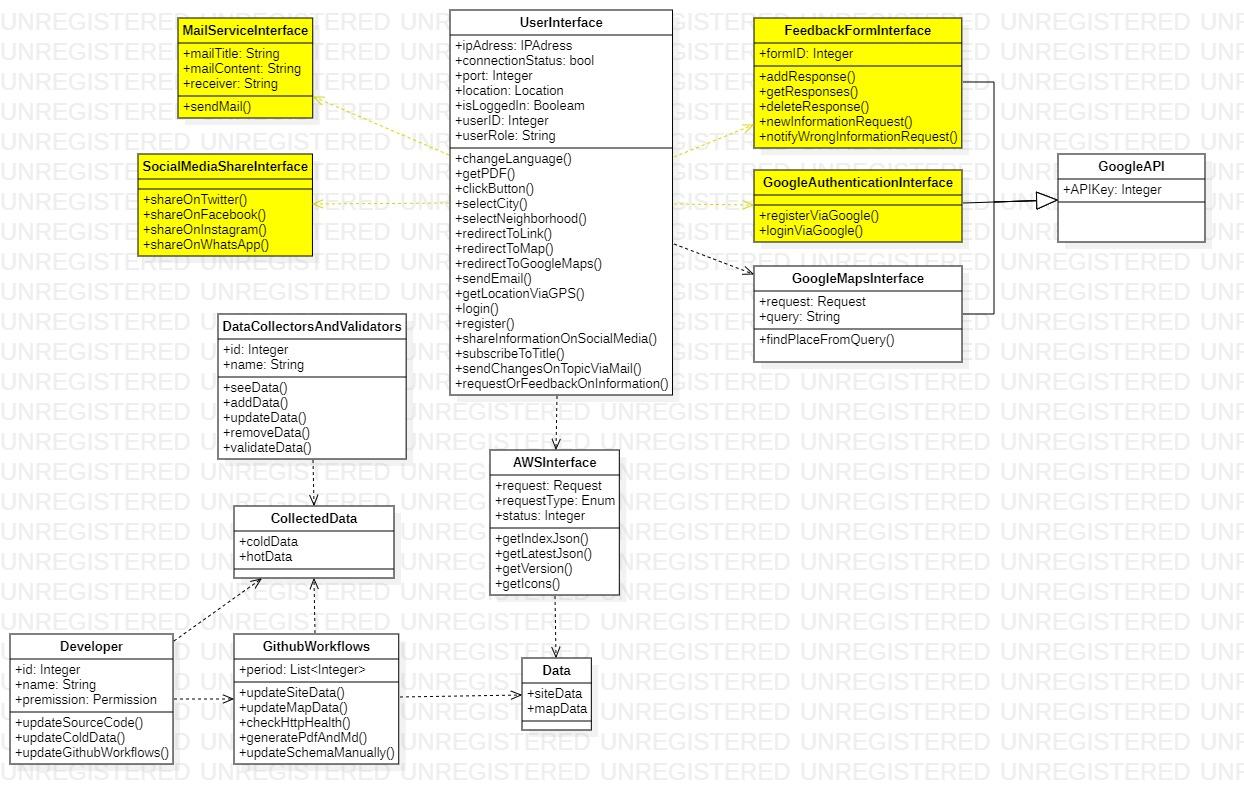
\includegraphics[width=\linewidth]{img/external-interfaces-s4.jpg}
  \caption{Suggested New External Interfaces}
\end{figure}
\vfill
\newpage

\subsection{Functions}

\subsection{Usability Requirements}

\subsection{Performance Requirements}

\subsection{Logical Database Requirements}

\afetbilgi\ does currently have a relational database. To make minor difference in the source code, the object structure in the Section 3.5 is preserved. Additionally, users, roles and mail subscription data are added into database. \texttt{Users} relation provides information related to the login system. \texttt{Roles} relation provides information related to the registered role. \texttt{Mail Subscription} relation provides the information related to topics that users subcribed. \texttt{SiteInformation} relation provides information related to the information located in the website.

\begin{figure}[H]
  \centering
  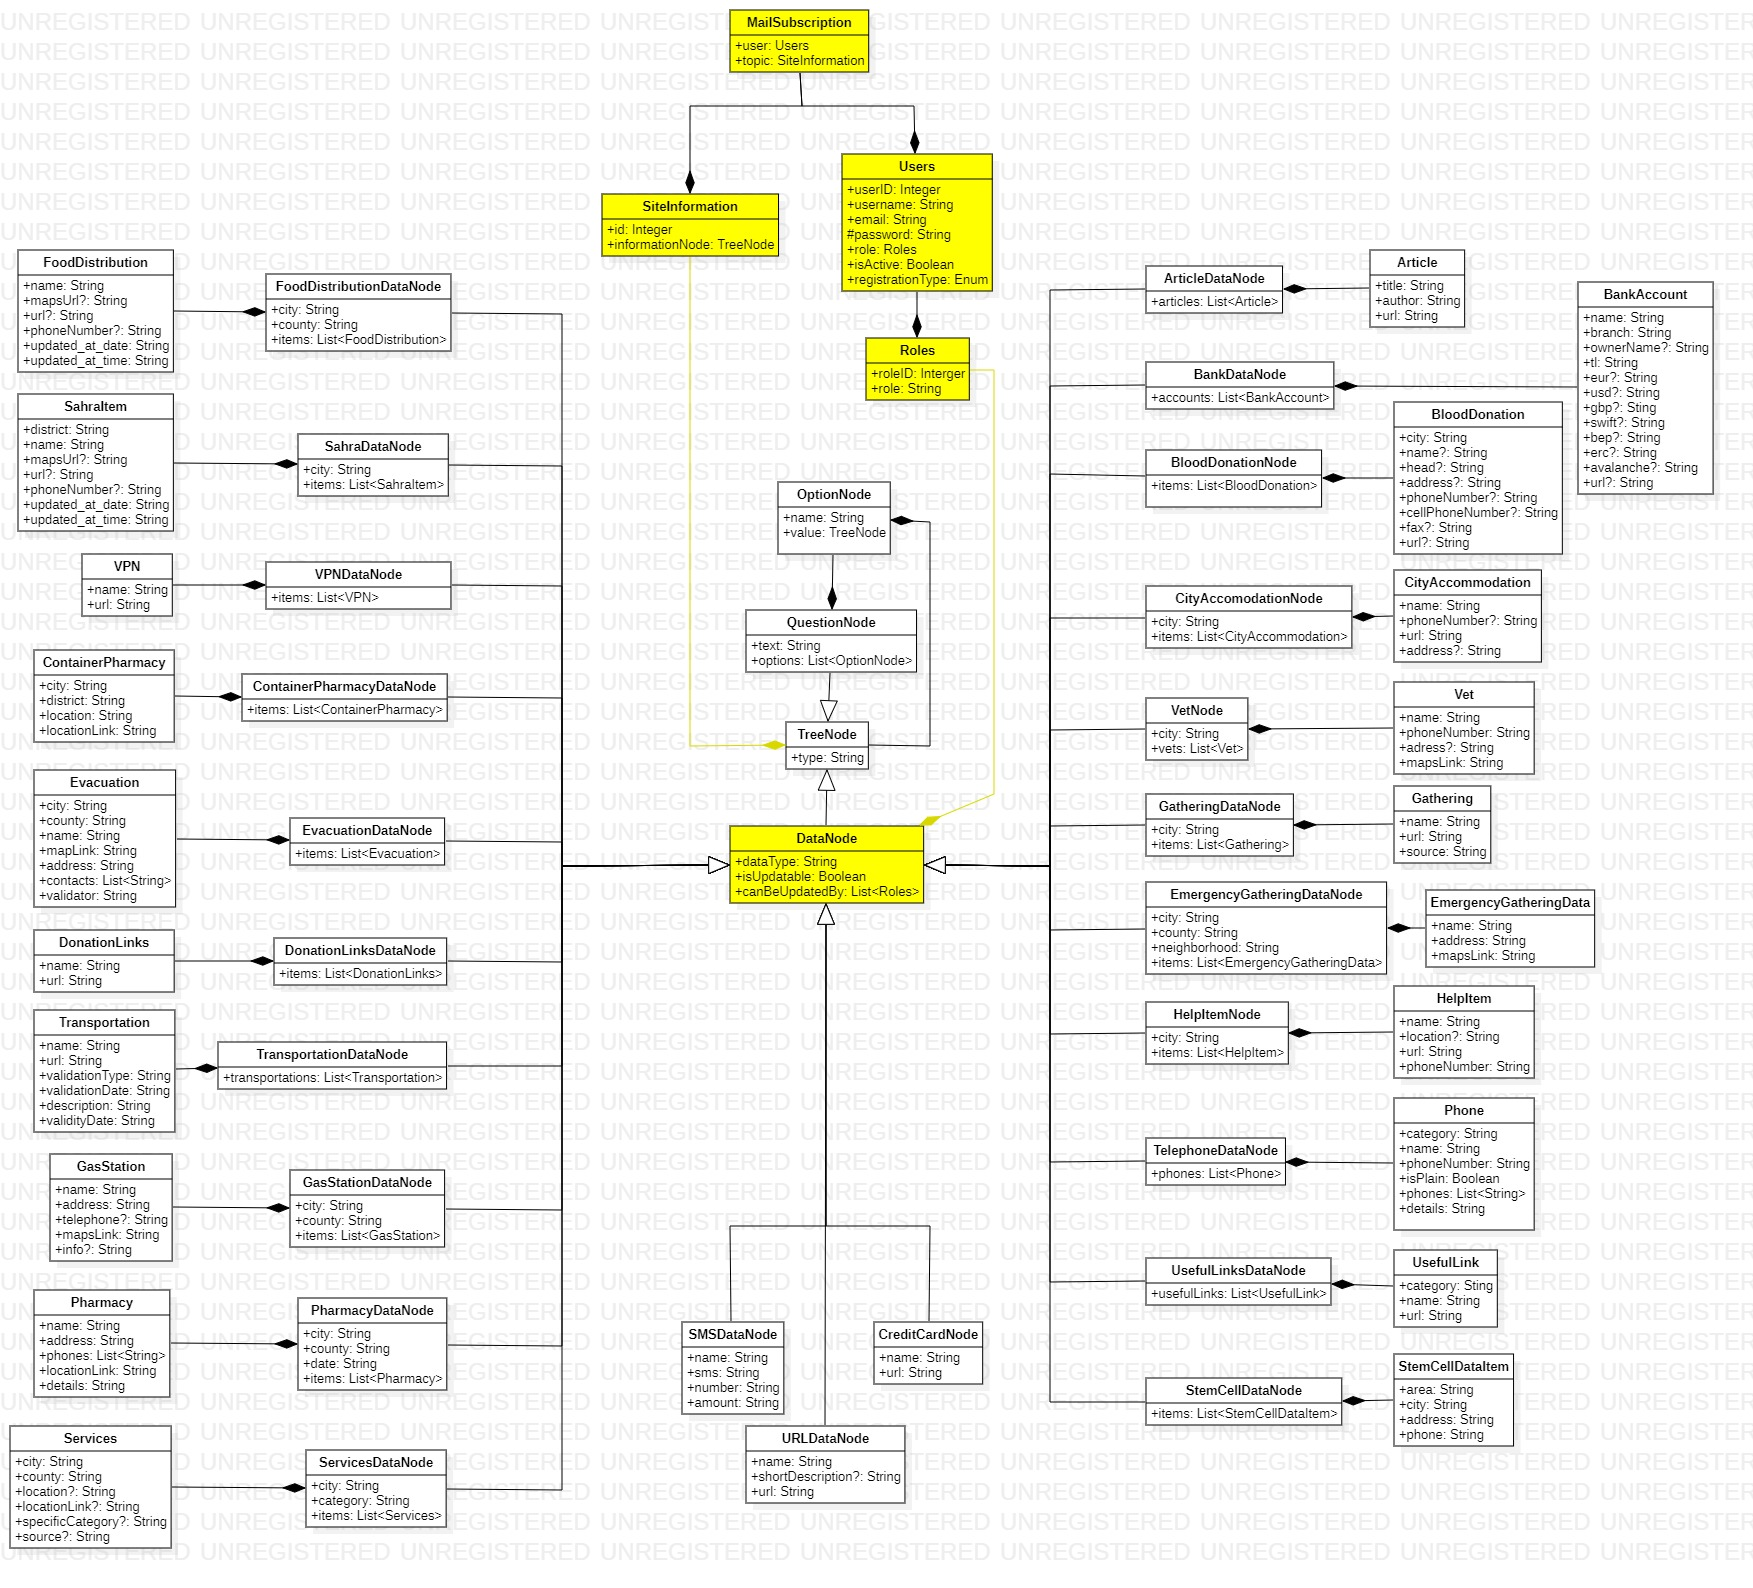
\includegraphics[width=\linewidth]{img/database-s4.jpg}
  \caption{Suggested New Relational Database}
\end{figure}

\subsection{Design Constraints}

\subsection{System Attributes}

\subsection{Supporting Information}
